%!TEX root=free234.tex
\begin{center}
    \bfseries\sffamily
    Space Curves\\
    \ttfamily worksheets/01space-curves.tex
\end{center}

\begin{trivlist}
\item[1] State the Frenet-Seret formulas.
\item[2] Here is a drawing of the space curve $\vx(t) = \tvek t\\t^2\\t^3\ttor$.

  Provided the missing annotations.  In particular, 
  \begin{trivlist}
  \item[a.] Label the axes 
  \item[b.] Find equations for the projected curves that are visible in the
    $xy$ or $xz$ or $yz$ planes.
  \item[c.] Draw unit tangent, normal and binormal at the origin.
  \item[d.] Draw the osculating plane.
  \end{trivlist}
\end{trivlist}

\begin{center}
  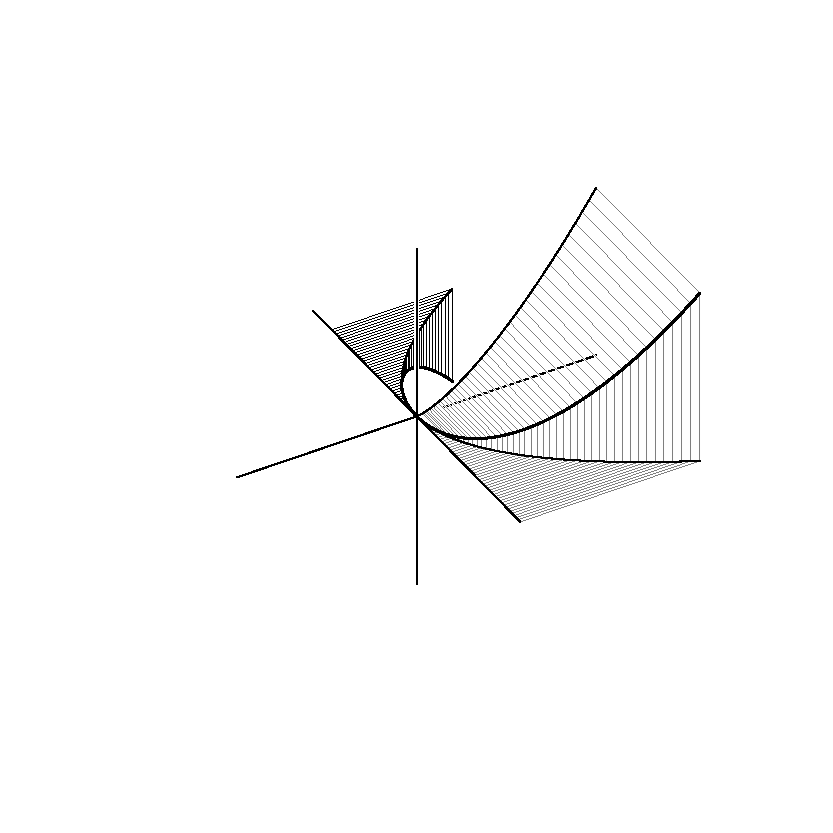
\includegraphics{figures/03osculating.pdf}
\end{center}
